\documentclass{standalone}
\usepackage{tikzducks}

\begin{document}
	
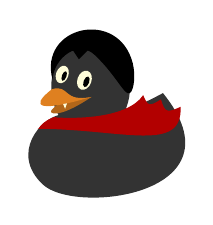
\begin{tikzpicture}
	\duck[body=black!80!white,laughing,cape=red!70!black,shorthair=black]
	\fill[white!85!yellow] (0.55,1.28) -- (0.575,1.22) -- (0.6,1.29) -- cycle;
	\fill[black] (0.65,2) -- (0.75,1.85) -- (0.9,2) -- cycle;
\end{tikzpicture}	
	
\end{document}